\documentclass[a4paper, 12pt]{article}

%%% Работа с русским языком
\usepackage{cmap}					% поиск в PDF
\usepackage{mathtext} 				% русские буквы в формулах
\usepackage[T2A]{fontenc}			% кодировка
\usepackage[utf8]{inputenc}			% кодировка исходного текста
\usepackage[russian]{babel}	% локализация и переносы

%%% Дополнительная работа с математикой
\usepackage{amsmath,amsfonts,amssymb,amsthm,mathtools} % AMS
\usepackage{icomma} % "Умная" запятая: $0,2$ --- число, $0, 2$ --- перечисление

%% Номера формул
%\mathtoolsset{showonlyrefs=true} % Показывать номера только у тех формул, на которые есть \eqref{} в тексте.

%% Шрифты
\usepackage{euscript}	 % Шрифт Евклид
\usepackage{mathrsfs} % Красивый матшрифт

%% Поля
\usepackage[left=2cm,right=2cm,top=2cm,bottom=2cm,bindingoffset=0cm]{geometry}

%% Русские списки
\usepackage{enumitem}
\makeatletter
\AddEnumerateCounter{\asbuk}{\russian@alph}{щ}
\makeatother

%%% Работа с картинками
\usepackage{graphicx}  % Для вставки рисунков
\graphicspath{{images/}{images2/}}  % папки с картинками
\setlength\fboxsep{3pt} % Отступ рамки \fbox{} от рисунка
\setlength\fboxrule{1pt} % Толщина линий рамки \fbox{}
\usepackage{wrapfig} % Обтекание рисунков и таблиц текстом

%%% Работа с таблицами
\usepackage{array,tabularx,tabulary,booktabs} % Дополнительная работа с таблицами
\usepackage{longtable}  % Длинные таблицы
\usepackage{multirow} % Слияние строк в таблице

%% Красная строка
\setlength{\parindent}{2em}

%% Интервалы
\linespread{1}
\usepackage{multirow}

%% TikZ
\usepackage{tikz}
\usetikzlibrary{graphs,graphs.standard}

%% Верхний колонтитул
\usepackage{fancyhdr}
\pagestyle{fancy}

%% Перенос знаков в формулах (по Львовскому)
\newcommand*{\hm}[1]{#1\nobreak\discretionary{}
	{\hbox{$\mathsurround=0pt #1$}}{}}

%% Мои дополнения
\usepackage{float} %Добавляет возможность работы с командой [H] которая улучшает расположение на странице
\usepackage{gensymb} %Красивые градусы
\usepackage{graphicx}               % Импорт изображений
\usepackage{caption} % Пакет для подписей к рисункам, в частности, для работы caption*
\usepackage{indentfirst}


\begin{document}

\newcommand{\HRule}{\rule{\linewidth}{0.7mm}} % Defines a new command for the horizontal lines, change thickness here
	
	\begin{center}
		\large\textbf{Московский Физико-Технический Институт}\\ % Name of your university/college
		\large\textbf{(государственный университет)}
	
		\vfill
		
		\Large Лабораторная работа по курсу общей физики № 4.5.3\\[0.5cm] % Preambule of your document title
		
		
		\HRule
		\\[0.4cm]
		{ \huge \bfseries Сканирующий интерферометр}% Title of your document
		\\[0.4cm] 
		\HRule
		\\[0.5cm]
		
		\ \\
	\textbf{\large Автор:} \\	
	\large Лепарский Роман Б01-003\\ % Your name and something more, your group num for example
		\vfill
		\hspace*{-0.8 cm}
\includegraphics[width=100 pt]{frkt_logo}\\ % logo of your  company/university/college
		\large Долгопрудный, 2022 % location and year
	\end{center}

\newpage
\setcounter{page}{2}
\fancyfoot[c]{\thepage}
\fancyhead[L] {Работа № 4.5.3} % some information in page header
\fancyhead[R]{}
\section{Аннотация}
\textbf{Цель работы:} изучить модели зрительных труб (астрономической
трубы Кеплера и земной трубы Галилея) и микроскопа, определить
их увеличения.

\textbf{Приборы и материалы:} оптическая скамья, набор линз, экран,
осветитель со шкалой, зрительная труба, диафрагма, линейка.

\section{Теоретические сведения}
	
	В работе предлагается измерить фокусные расстояния линз, смоделировать трубу Кеплера, трубу Галилея, микроскоп и определить их увеличения. Предметом служит миллиметровая сетка, нанесённая на матовое стекло осветителя.
	
	При юстировке любых оптических приборов важно правильно центрировать входящие в систему линзы. Проходя через плохо отцентрированную систему линз, лучи света отклоняются в сторону и могут вообще не доходить до глаза наблюдателя.
	
	Для построения телескопических систем необходим удаленный объект. Эту роль выполняет коллиматор настроенный на бесконечность.
	
	Фокусные расстояния положительных линз проще всего найти с помощью вспомогательной зрительной трубы, установленной на бесконечность. 
	
	\subsection{Определение фокусных расстояний тонких линз с помощью
		зрительной трубы}
	\begin{figure}[H]
		\centering
		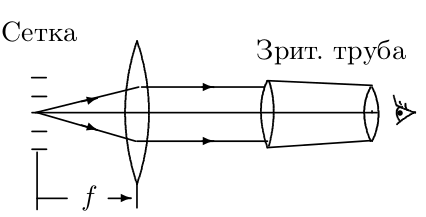
\includegraphics[scale=0.7]{focus}
	\end{figure}

	Определение фокусного расстояния линзы происходит с помощью зрительной трубы настроенной на бесконечность. Так как лучи от сетки, расположенной в фокусе после прохождения положительной линзы идут параллельно. А чтобы достичь того же эффекта от отрицательной линзы, нужно разместить перед ней собирающую.
	
	\begin{figure}[H]
		\centering
		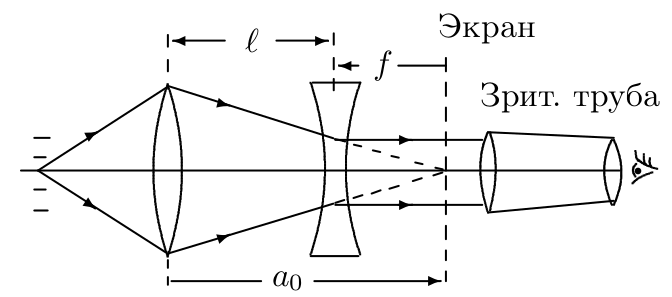
\includegraphics[scale=0.5]{focus2}
	\end{figure}

	\subsection{Телескоп Кеплера}
	
	\begin{figure}[H]
		\centering
		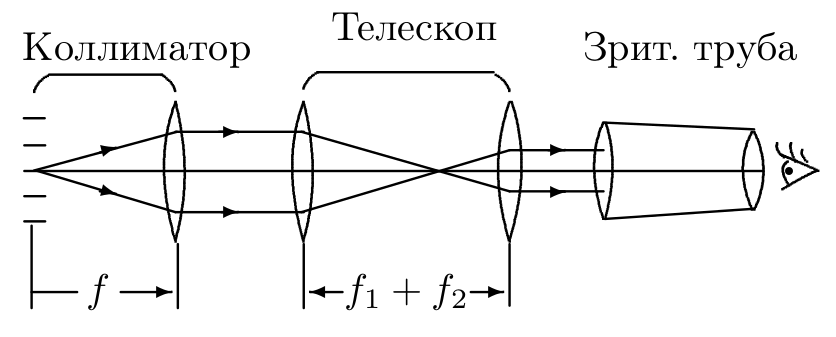
\includegraphics[scale=0.4]{kepler}
	\end{figure}

	Увеличение этой модели телескопа рассчитывается по формуле
	\[
		\Gamma_K = -\frac{f_1}{f_2}
	\]
	Или для телесных углов
	\[
	\Gamma_K = -\frac{h_2}{h_1}
	\]
	Или для диаметра диафрагмы
	\[
	\Gamma_K = -\frac{D_1}{D_2}
	\]
	
	\subsection{Труба Галилея}
		
	Данная оптическая система отличается от трубы Кеплера только тем, что в качестве окуляра берется рассеивающая линза.
	
	\begin{figure}[H]
		\centering
		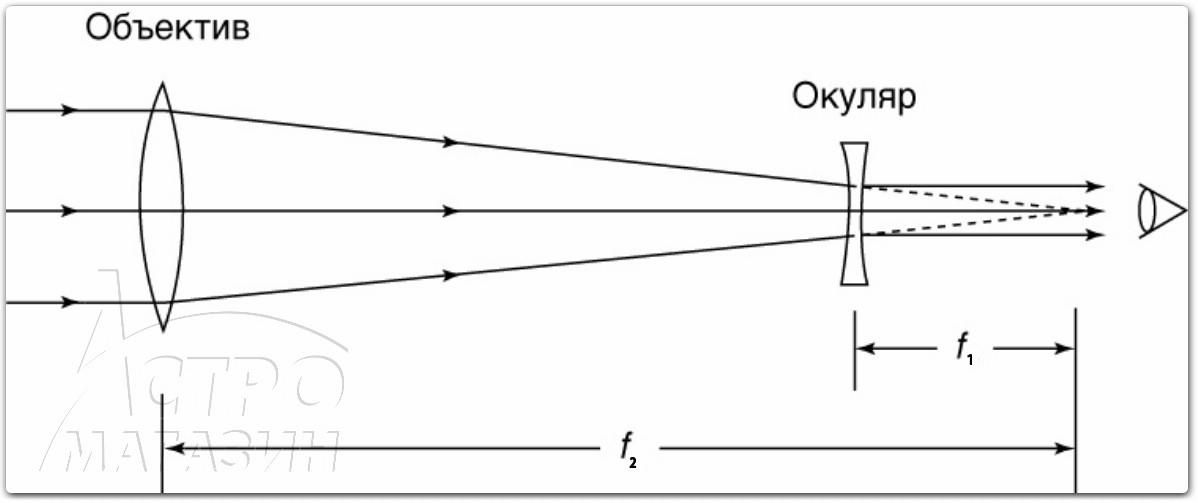
\includegraphics[scale=0.3]{gal}
	\end{figure}

	\subsection{Модель микроскопа}
	
	Оптическая схема микроскопа выглядит следующим образом
	\begin{figure}[H]
		\centering
		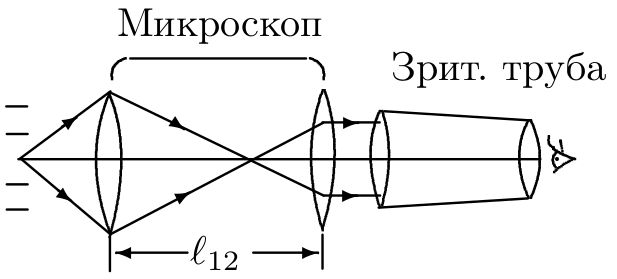
\includegraphics[scale=0.5]{micro}
	\end{figure}

	Его увеличение можно найти так
	\[
		\Gamma_M = \frac{h_2L}{h_1f}
	\]
	где $f$ - фокусное расстояние коллиматорной линзы, используемой для измерения $h_1$, А $L = 25$ см - расстояние наилучшего зрения.
	
	\section{Обработка результатов}
	После центрировки оптической системы найдем фокусные расстояния собирающих линз.
	\subsection{Определение фокусных расстояний тонких линз}
	Отберем из набора собирающие линзы и с помощью схемы 2.1 определим их фокусное расстояние. Погрешность обусловлена невозможностью определить точное положение линзы внутри оправы.
	
	\begin{table}[H]
		\centering
		\begin{tabular}{|l|l|l|l|l|}
			\hline
			$N$ & $f_1^+$, см  & $f_2^+$, см  & $f^+$, см & $\sigma_{f}$, см \\ \hline
			1   & $7,6\pm0,2$  & $7,5\pm0,2$  & $7,55$    & 0,14             \\ \hline
			2   & $10,5\pm0,2$ & $10,6\pm0,2$ & $10,55$   & 0,14             \\ \hline
			3   & $19,2\pm0,3$ & $18,9\pm0,3$ & $19,1$    & 0,2              \\ \hline
			4   & $28,2\pm0,3$ & $28,0\pm0,3$ & $28,1$    & 0,2              \\ \hline
		\end{tabular}
	\end{table} 
	Погрешность определим по формуле косвенных измерений
	\[
		\sigma_f = \sqrt{\left(\frac{\sigma_+}{2}\right)^2+\left(\frac{\sigma_-}{2}\right)^2}
	\]
	
	Чтобы определить фокусное расстояние рассеивающей линзы поместим собирающую после источника и найдем расстояние до изображения $a_0 = 34,4\pm0,2$ см. Тогда фокусное расстояние собирающей линзы:
	\begin{table}[H]
		\centering
		\begin{tabular}{|l|l|l|l|l|}
			\hline
			$N$ & $l_1^-$, см  & $l_2^-$, см  & $l^-$, см    & $f^-$, см   \\ \hline
			5   & $27,9\pm0,3$ & $27,7\pm0,3$ & $27,8\pm0,2$ & $-6,6\pm0,1$ \\ \hline
		\end{tabular}
	\end{table}

	\subsection{Телескоп Кеплера}
	В качестве коллиматора возьмем линзу №3 ($f=19,1$ см), сам телескоп соберем из линз 4 и 2 ($f_1=28,1$ см, $f_2=10,55$ см).
	
	Запишем данные для определения увеличения:
	\begin{table}[H]
		\centering
		\begin{tabular}{|l|l|l|l|}
			\hline
			$h_1$, дел   & $h_2$, дел & $D_1$, мм & $D_2$, мм  \\ \hline
			$10,0\pm0,5$ & $28\pm1$   & $36\pm1$  & $13\pm0,5$ \\ \hline
		\end{tabular}
	\end{table}
	и определим увеличение разными способами
	\[
		\Gamma_K=-\frac{f_1}{f_2} = -2,66\pm0,04
	\]
	\[
		\Gamma_K=-\frac{h_2}{h_1} = -2,8\pm0,17
	\]
	\[
		\Gamma_K=-\frac{D_1}{D_2} = -2,7\pm 0,13
	\]
	Погрешность формул вида $x/y$ рассчитывается по формуле
	\[
		\sigma = \sqrt{\left(\frac{\sigma_x}{y}\right)^2 + \left(\frac{x\sigma_y}{y^2}\right)^2}
	\]
	Видно, что результаты сходятся в пределах погрешности.
	
	\subsection{Труба Галилея}
	В качестве объектива и коллиматора оставим те же линзы, что и в предыдущем опыте. А в качестве окуляра возьмем рассеивающую линзу ($f = -6,6$ см).
	
	Запишем результаты измерений.
	\begin{table}[H]
		\centering
		\begin{tabular}{|l|l|}
			\hline
			$h_1$, дел   & $h_2$, дел \\ \hline
			$10,0\pm0,5$ & $42\pm2$   \\ \hline
		\end{tabular}
	\end{table}

	\[
		\Gamma_G = -\frac{f_1}{f_2} = 4,25\pm0,07
	\]
	\[
		\Gamma_G = \frac{h_2}{h_1} = 4,2\pm 0,2
	\]
	Результаты сходятся в пределах погрешности.
	
	\subsection{Модель микроскопа}
	Для этой модели отберем из набора линзы ($f_1 = 7,55$ см) и ($f_2 = 10,55$ см). Желаемое увеличение $\Gamma_M = 5$. Согласно формуле $\Gamma_M = \dfrac{\Delta L}{f_1f_2}$ и $\Delta = l_{12} - f_1 - f_2$. Найдем длину тубуса $l_{12} = 34$ см.
	
	Измерим величину изображения миллиметрового деления предметной шкалы. $h_2 \hm= 37\pm1$ дел. И найдем увеличение микроскопа по формуле
	\[
		\Gamma_M = -\frac{h_2L}{h_1f} = 4,8\pm2
	\]
	\[
		\sigma_M = \sqrt{\left(\frac{\sigma_{h_2}L}{h_1f}\right)^2 + \left(\frac{\sigma_{h_1}h_2L}{h_1^2f}\right)^2+ \left(\frac{\sigma_{f}h_2L}{h_1f^2}\right)^2}
	\]
	Хотя, формально желаемый результат попадает в погрешность, отличие все же значительное. Это может быть связано со сложностью установления длины тубуса согласно рассчитанному значению.
	\section{Вывод}
	В этой работе мы исследовали модели зрительных труб и микроскопа, а так же определили их увеличения различными способами.
	
	
	
	
	
	
	
	
	
	
	
	
	
	
	
	
	
	
	

\end{document}